\chapter[Incompressible flow equations]{Incompressible flow equations}
\label{ch:ch2incompeq}

%% The following annotation is customary for chapter which have already been
%% published as a paper.
%\blfootnote{This chapter has been submitted to the Journal of Fluid Mechanics.}
%\blfootnote{footnote}
\begin{abstract}
In this chapter the governing equations and solution methods for incompressible flows are presented. The incompressible Navier Stokes equations are first given in dimensional and non-dimensional forms. Subsequently, the finite volume method applied to a general conservation equation is described. The difficulty associated with solving the incompressible flow equations numerically, namely the pressure velocity coupling, is described and the different methods to overcome this issue are presented. Finally, the solution procedure to solve turbulent incompressible flow equations are shown.
\end{abstract}
%This chapter presents the governing equations for incompressible flow and describes  different solution methods. 
\section{Navier Stokes equations}
The governing flow equations for incompressible flow with constant density and viscosity and no heat transfer are 
\begin{equation}
\frac{\partial (\rho u)}{\partial x} + \frac{\partial (\rho v)}{\partial y} + \frac{\partial (\rho w)}{\partial z} = 0,
\label{eq:continuity}
\end{equation}
\begin{equation}
\frac{\partial (\rho u)}{\partial t} + \frac{\partial (\rho u u)}{\partial x}+ \frac{\partial (\rho uv)}{\partial y} + \frac{\partial (\rho uw)}{\partial z} = -\frac{\partial p}{\partial x} + \mu\left(\frac{\partial^2 u}{\partial x^2} + \frac{\partial^2 u}{\partial y} + \frac{\partial^2 u}{\partial z}\right)
\label{eq:xmommentum}
\end{equation}
\begin{equation}
\frac{\partial (\rho v)}{\partial t} + \frac{\partial (\rho uv)}{\partial x}+ \frac{\partial (\rho vv)}{\partial y} + \frac{\partial (\rho vw)}{\partial z} = -\frac{\partial p}{\partial y} + \mu\left(\frac{\partial^2 v}{\partial x^2} + \frac{\partial^2 v}{\partial y} + \frac{\partial^2 v}{\partial z}\right)
\label{eq:ymommentum}
\end{equation}
\begin{equation}
\frac{\partial (\rho w)}{\partial t} + \frac{\partial (\rho wu)}{\partial x}+ \frac{\partial (\rho wv)}{\partial y} + \frac{\partial (\rho ww)}{\partial z} = -\frac{\partial p}{\partial z} + \mu\left(\frac{\partial^2 w}{\partial x^2} + \frac{\partial^2 w}{\partial y} + \frac{\partial^2 w}{\partial z}\right)
\label{eq:zmommentum}
\end{equation}
where $\rho$ is the constant density of the fluid, $u$, $v$ and $w$ are the $x-$, $y-$ and $z-$ components of the velocity vector respectively, $p$ is the pressure and $\mu$ is the dynamic viscosity, assumed to be constant. Equation~\ref{eq:continuity} is the continuity equation or the mass conservation equation. For incompressible flows, this condition reduces to a zero divergence condition for the velocity vector. Equations~\ref{eq:xmommentum}, \ref{eq:ymommentum} and \ref{eq:zmommentum} are the momentum conservation equations in $x$, $y$ and $z$ directions respectively. Here it is assumed that the fluid is Newtonian. Under the incompressible flow assumption the energy equation is decoupled from the continuity and momentum equations and is therefore not shown here.
\subsection{Non-dimensionalization}
All the quantities in equations~\ref{eq:continuity}, \ref{eq:xmommentum}, \ref{eq:ymommentum} and \ref{eq:zmommentum} are dimensional and their magnitudes can vary widely. The governing equations can be transformed into a non dimensional form by scaling the variables using reference values. The scaling parameters can be defined as follows
\begin{list}{}{}
	\item $L$ - reference length (e.g. chord of the airfoil),
	\item $V$ - reference velocity (e.g. the free stream velocity, $V_{\infty}$),
	\item $f$ - characteristic frequency (e.g., one cycle of a periodic process, or $V/L$),
	\item $p_0$ - reference pressure (e.g., dynamic pressure, $\rho V_{\infty}^2$).
\end{list}

With the aid of these characteristic quantities we can define the following non-dimensional variables
\begin{equation*}
	x^*=\frac{x}{L}, \quad y^*=\frac{y}{L}, \quad z^*=\frac{z}{L},
\end{equation*}
\begin{equation*}
	u^*=\frac{u}{V}, \quad v^*=\frac{v}{V}, \quad w^*=\frac{w}{V},
\end{equation*}
\begin{equation*}
	p^*=\frac{p}{p_0}=\frac{p}{\rho V^2}, \quad t^*= tf.
\end{equation*}
Based on dimensional analysis, the following non dimensional numbers can be defined
\begin{equation}
St = \frac{fL}{V}, \label{eq:Stdefn} 
\end{equation}
\begin{equation}
Re = \frac{V L}{\nu} , \label{eq:Redefn}
\end{equation}
where $St$ is known as the Strouhal number and $Re$ is the Reynolds number. $\nu=\frac{\mu}{\rho}$ is the kinematic viscosity. Using the non-dimensional variables and the new non dimensional numbers, equation~\ref{eq:continuity} can be written as:
\begin{equation*}
\frac{\partial u^*}{\partial x^*} + \frac{\partial v^*}{\partial y^*} + \frac{\partial w^*}{\partial z^*}= 0,
\end{equation*}
and the equations~\ref{eq:xmommentum}, \ref{eq:ymommentum} and \ref{eq:zmommentum} as 
\begin{equation*}
St \frac{\partial u^*}{\partial t^*} + \frac{\partial (u^* u^*)}{\partial x^*} +  \frac{\partial (u^* v^*)}{\partial y^*} + \frac{\partial (u^* w^*)}{\partial z^*} = -\frac{p_0}{\rho V^2}\frac{\partial p^*}{\partial x*} + \frac{1}{Re}\left( \frac{\partial^2 u^*}{\partial x^{*2}} + \frac{\partial^2 u^*}{\partial y^{*2}} + \frac{\partial^2 u^*}{\partial z^{*2}}\right),
\end{equation*}
\begin{equation*}
St\frac{\partial v^*}{\partial t^*} + \frac{\partial (v^*u^*)}{\partial x^*} + \frac{\partial (v^*v^*)}{\partial y^*} +\frac{\partial (v^*w^*)}{\partial z^*} = -\frac{p_0}{\rho V^2}\frac{\partial p^*}{\partial y*} + \frac{1}{Re}\left( \frac{\partial^2 v^*}{\partial x^{*2}} + \frac{\partial^2 v^*}{\partial y^{*2}} + \frac{\partial^2 v^*}{\partial z^{*2}}\right),
\end{equation*}
\begin{equation*}
St\frac{\partial w^*}{\partial t^*} + \frac{\partial (w^*u^*)}{\partial x^*} + \frac{\partial (w^*v^*)}{\partial y^*} +\frac{\partial (w^*w^*)}{\partial z^*} = -\frac{p_0}{\rho V^2}\frac{\partial p^*}{\partial z*} + \frac{1}{Re}\left( \frac{\partial^2 v^*}{\partial x^{*2}} + \frac{\partial^2 v^*}{\partial y^{*2}} + \frac{\partial^2 v^*}{\partial z^{*2}}\right).
\end{equation*}
If the reference values are chosen judiciously, the comparison of the different non dimensional quantities can yield information about the relative importance of different flow features. Additionally, matching the non dimensional parameters will allow for comparison of data across different experiments and numerical simulations. 

The above equations can be written more compactly using the index notation (see below). In addition to using the index notation, the time and pressure references are chosen as $f = V/L$ and $p_0 = \rho V^2$ leading to the coefficients of the unsteady term and the pressure gradient term to be unity. The $\ast$ is dropped for the sake of convenience but all quantities shown are non dimensional.
\begin{equation}
\frac{\partial u_i}{\partial x_i} = 0,
\label{eq:contindx}
\end{equation}
\begin{equation}
\frac{\partial u_i}{\partial t} + \frac{\partial (u_iu_j)}{\partial x_j} = -\frac{\partial p}{\partial x_i} + \frac{1}{Re}\left( \frac{\partial^2 u_i}{\partial x_j\partial x_j} \right).
\label{eq:momindx}
\end{equation}
Here the velocities are represented by $u_i$, with $i=1,2,3$ being the three components of the velocity vector and similarly $x_i$ represents the three coordinate directions. Repeated indices indicate a summation over that index. Thus, equation~\ref{eq:momindx} represents the three momentum equations.

The rest of the thesis will use index notation to keep the equations compact.

\section{Numerical methods}
%Describe numerical methods - briefly introduce FVM and show discretization.
The equations described in the previous section cannot be solved analytically except for some simplified cases and are solved numerically. Consider the example of a typical flow problem - the flow past a cylinder. The region of interest extends outwards from the cylinder as shown in figure~\ref{fig:airfoildom}. 
\begin{figure}[h!]
\centering
\captionsetup{justification=centering}
 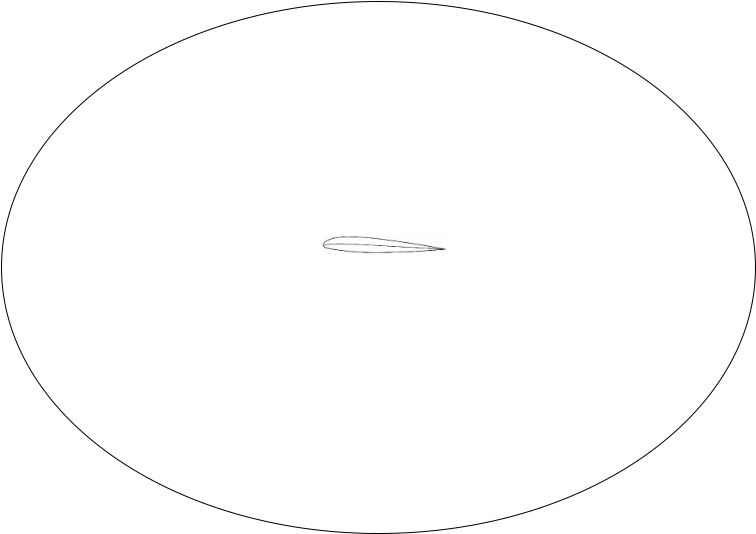
\includegraphics[width=0.55\textwidth]{ch2_litsurvey/Figures/airfoil_domain.png}
\caption{Region of interest for flow over a cylinder.}
 \label{fig:airfoildom}
\end{figure} 
In order to find the velocities and pressures in this region, the physical domain is divided into smaller domains where the partial differential equations can be approximated in a simpler manner. This process is known as \textit{discretization}. Since the partial differential equations are non-linear, care must be taken during the discretization process to preserve all the important flow phenomena in the approximate equations as well. 

However, in order to solve the approximate equations numerically, they must converted into algebraic equations. The equations are then solved at some specified points (\textit{nodes} or \textit{grid points}) within each of the smaller domains. This process can be done using many different methods. The earliest approaches used truncated Taylor series approximations of the difference terms known as the finite difference method. A more common approach is the finite volume method where the governing equations are integrated over the smaller discretized regions to obtain an approximate algebraic equation. In this study, the finite volume discretization is used. More information about other discretization techniques can be found in literature (for example~\cite{Moukalled,hirsch1997numerical,Ferziger2002}).
\subsection{Finite Volume discretization}\label{sec:ch2disceqnphi}
In this section the finite volume discretization methods will be described briefly. 
Consider a general conservation equation for any scalar variable $\phi$ 
\begin{equation}
\frac{\partial (\rho \phi)}{\partial t} + \frac{\partial (\rho U_i \phi)}{\partial x_i} = \frac{\partial}{\partial x_i}\left(\Gamma\frac{\partial \phi}{\partial x_i}\right) + Q
\label{eq:genphi}
\end{equation}
where $\rho$ is the constant fluid density, $U_i$ is the velocity field (assumed constant in this section), $\Gamma$ is the diffusion coefficient and $Q$ is a source term. First, the physical domain on which the equation~\ref{eq:genphi} needs to be solved is discretized into smaller domains known as \textit{control volumes}. For simplicity consider a $2D$ case and define a control volume around a node $P$ as shown in figure~\ref{fig:2ddaxis}.
\begin{figure}[h]
\centering
\captionsetup{justification=centering}
 \includegraphics[width=0.4\textwidth]{ch2_litsurvey/Figures/2ddomainwaxisneigh.png}
\caption{$2D$ control volume around a node $P$.}
 \label{fig:2ddaxis}
\end{figure} 

The control volume is bound on four sides by faces $e$, $w$, $n$ and $s$  representing east, west, north and south respectively. Integrating equation~\ref{eq:genphi} on a control volume $\Omega$ gives
\begin{equation}
\int_{\Omega}\frac{\partial (\rho \phi)}{\partial t}d\Omega + \int_{\Omega} \frac{\partial (\rho U_i \phi)}{\partial x_i} d\Omega = \int_{\Omega}\frac{\partial}{\partial x_i}\left(\Gamma\frac{\partial \phi}{\partial x_i}\right) d\Omega + \int_{\Omega} Q d\Omega.
\label{eq:genphidisc}
\end{equation}

\subsubsection{Discretization of the viscous term}
First consider the diffusion term on the right hand side of equation~\ref{eq:genphidisc}. Using the divergence theorem the volume integral can be converted into a surface integral as
\begin{equation}
\int_{\Omega}\frac{\partial}{\partial x_i}\left(\Gamma\frac{\partial \phi}{\partial x_i}\right) d\Omega = \int_{\partial \Omega} \left(\Gamma\frac{\partial \phi}{\partial x_i}\right) n_i d (\partial\Omega),
\end{equation}
where $\partial \Omega$ represents the boundary of the control volume and $n_i$ is the unit outward pointing normal of the boundary. In the simplified $2D$ example of figure~\ref{fig:2ddaxis}, 
%the boundary of the control volume consists of the faces $e$, $w$, $n$ and $s$ and thus 
the integral can be written as a summation over the four faces as
\begin{equation}
\int_{\partial \Omega} \left(\Gamma\frac{\partial \phi}{\partial x_i}\right) n_i d (\partial\Omega) = \sum_{f} \left(\Gamma\frac{\partial \phi}{\partial x_i}\right) n_i \Delta S_f,
\end{equation}
where $f=e,w,n$ and $s$, $n_i$ is the corresponding outward unit normal vector of the face $f$ and $\Delta S_f$ is the area of the face $f$. Here the midpoint integration rule is used and the quantities on the face $f$ are computed at the face centroids. Based on the axis directions shown in figure~\ref{fig:2ddaxis} the summation can be expanded as
\begin{align}
\sum_{f} \left(\Gamma\frac{\partial \phi}{\partial x_i}\right) n_i \Delta S_f = \left(\Gamma\frac{\partial \phi}{\partial x_1}\right)_e \Delta S_e - 
\left(\Gamma\frac{\partial \phi}{\partial x_1}\right)_w \Delta S_w + \nonumber \\
\left(\Gamma\frac{\partial \phi}{\partial x_2}\right)_n \Delta S_n -
\left(\Gamma\frac{\partial \phi}{\partial x_2}\right)_s \Delta S_s.
\label{eq:viscsumm}
\end{align}
Here $x_1$ and $x_2$ are the $x$ and $y$ directions respectively. The derivatives at the faces can be written based on the nodal values of $\phi$. For example, considering the neighboring nodes to east of node $P$ in figure~\ref{fig:2ddaxis} to be $E$, the derivative of $\phi$ at the face $e$ for a constant $\Gamma$ can be written as
\begin{equation}
\left(\Gamma\frac{\partial \phi}{\partial x_1}\right)_e \Delta S_e = \Gamma \frac{\phi_E-\phi_P}{\Delta_{PE}}\Delta S_e = a_{E,v}\phi_E - a_{E,v}\phi_P,
\end{equation}
where $\Delta_{PE}$ is the distance between the nodes $P$ and $E$ and $a_{E,v}$ is the viscous coefficient of $\phi_E$ given by
\begin{equation*}
a_{E,v} = \Gamma \frac{\Delta S_e}{\Delta_{PE}}.
\end{equation*}
Similar expressions can be written for the other terms in the summation in equation~\ref{eq:viscsumm} to obtain an algebraic relation in terms of the nodal values of $\phi$ with the viscous coefficients being
\begin{equation*}
a_{W,v} = \Gamma \frac{\Delta S_w}{\Delta_{PW}}, \quad a_{N,v} = \Gamma \frac{\Delta S_n}{\Delta_{PN}}, \quad a_{S,v} = \Gamma \frac{\Delta S_s}{\Delta_{PS}},
\end{equation*}
and
\begin{equation*}
a_{P,v} = -(a_{E,v} + a_{W,v} + a_{N,v} + a_{S,v}).
\end{equation*}
Here $a_{P,v}$ is the viscous coefficient of $\phi_{P}$.
\subsubsection{Discretization of the advective term}
Now focusing on the advective term of equation~\ref{eq:genphidisc} and applying the divergence theorem again gives,
\begin{equation}
\int_{\Omega} \frac{\partial (\rho U_i \phi)}{\partial x_i} d\Omega = \int_{\partial \Omega} \rho U_i \phi n_i d(\partial \Omega).
\end{equation}
Similar to the discretization of the viscous term, the surface integral can be split into a summation over the four bounding faces of the control volume shown in figure~\ref{fig:2ddaxis}
\begin{equation*}
\int_{\partial \Omega} \rho U_i \phi n_i d(\partial \Omega) = \sum_f \left(\rho U_i \phi n_i \right)_f \Delta S_f,
\end{equation*}
\begin{equation*}
\sum_f \left(\rho U_i \phi n_i \right)_f \Delta S_f = \left(\rho U_1 \phi \right)_e \Delta S_e - \left(\rho U_1 \phi \right)_w \Delta S_w + \left(\rho U_2 \phi \right)_n \Delta S_n - \left(\rho U_2 \phi \right)_s \Delta S_s,
\end{equation*}
where the same sign convention used for the viscous discretization is also applied here and the mid point integration rule is used to approximate the integral over the face. The  term within the brackets can be found using the known velocity field. Determining the value of the scalar variable, $\phi$, can be done in various ways. Some of the more common methods are described below.
\begin{figure}[h]
\centering
\captionsetup{justification=centering}
 \includegraphics[width=0.3\textwidth]{ch3_su2eqn/figures/1dcv.png}
\caption{$1D$ control volume around node $P$ and neighboring nodes $E$ and $W$.}
 \label{fig:ch2pefrcinterp}
\end{figure}
\paragraph{Central scheme}
In a central scheme, the value of the scalar variable is approximated as the weighted average of the neighboring nodes. For example at the face $e$ and assuming the eastward neighbor of node $P$ in figure~\ref{fig:ch2pefrcinterp} is $E$, the value of $\phi$ is simply
\begin{equation}
\phi_e = \lambda_P \phi_P + \lambda_E \phi_E,
\end{equation}
where $\lambda_P$ and $\lambda_E$ are weighting factors of $P$ and $E$ respectively given by
\begin{equation}
\lambda_P = \frac{d_{Pe}}{d_{PE}}, \quad \lambda_E = \frac{d_{eE}}{d_{PE}}.
\end{equation} 
Here $d_{Pe}$ is the distance from node $P$ to face $e$, $d_{eE}$ is the distance from face $e$ to node $E$ and $d_{PE}$ is the distance from node $P$ to node $E$ ($d_{PE} = d_{Pe} + d_{eE}$). Thus, the contribution from the face $e$ to the summation can be written in terms of the nodal values of $\phi$ as 
\begin{equation}
\left(\rho U_i \phi \right)_e \Delta S_e = (\rho U_1 \Delta S)_e \lambda_P \phi_P + (\rho U_1 \Delta S)_e\lambda_E \phi_E.
\end{equation}
Hence,
\begin{equation*}
a_{E,c} = (\rho U_1 \Delta S)_e\lambda_E.
\end{equation*}
Similarly for the other faces around the control volume of node $P$ in figure~\ref{fig:2ddaxis}, the coefficients of the nodal values of $\phi$ can be written as
\begin{equation*}
a_{W,c} = -(\rho U_1 \Delta S)_w\lambda_W, \quad a_{N,c} = (\rho U_2 \Delta S)_n\lambda_N, \quad a_{S,c} = -(\rho U_2 \Delta S)_s\lambda_S,
\end{equation*}
and as with the viscous term discretization,
\begin{equation*}
a_{P,c} = -(a_{E,c} + a_{W,c} + a_{N,c} + a_{S,c}).
\end{equation*}
\paragraph{Upwind scheme}
An alternative to the central scheme, is to mimic the physics of the problem and determine the value at the face based on the direction of flow. 
Denoting the term
\begin{equation*}
\rho U_i n_i \Delta S_f = \dot{m}_f,
\end{equation*}
as the mass flux across the face $f$, the direction of the flow can be found based on the sign of the mass flux. Choosing the value of $\phi$ as
\begin{equation}
\phi_e = \begin{cases}
\phi_P\quad if\quad \dot{m}_e > 0, \\
\phi_E\quad if\quad \dot{m}_e < 0,
\end{cases}
\end{equation}
will replicate the physics of the flow at the face $e$. If the flow is in the positive $x$ direction, the mass flux at the face $e$ is positive ($\dot{m}_e>0$) and the value of the variable at the node $P$ is chosen. On the other hand if the direction of the flow is reversed, the value of $\phi$ at the node $E$ is chosen. This ensures the physics of the flow is also replicated in the discretized equation. The coefficients of the nodal values of $\phi$ for the face $e$ are then
\begin{equation}
a_{E,c} = \text{max}(-m_e,0.0), \quad a_{P,c} = \text{max}(m_e,0.0).
\end{equation}
Similar expressions can be written at other faces to find the coefficients of $\phi_P$ and its neighbors.

To examine the difference in behavior of the central and upwind scheme, consider a one dimensional pure advection problem given by
\begin{equation}
\frac{\partial \rho \phi}{\partial t} + \frac{\partial (\rho U \phi)}{\partial x} = 0.
\label{eq:advecphieqn}
\end{equation}
Let the domain of the problem be $x \in [0,1]$ and $U=1$ is the advection velocity and $\rho=1$ is the density. Assume an initial condition for $\phi$ as
\begin{equation}
\phi_0 = \begin{cases}
1.0 \quad if \quad x < 0.25, \\
0 \quad if \quad x > 0.25.
\end{cases}
\end{equation}
Since no dissipation is present, the initial condition must be advected across the domain without any loss in information. Figure~\ref{fig:upwcen} shows the numerical results from both the upwind and central schemes compared against the exact solution.
\begin{figure}[h]
\centering
\captionsetup{justification=centering}
 \includegraphics[trim=0 390 0 0,clip, width=0.5\textwidth]{ch2_litsurvey/Figures/box_cen_fo.eps}
\caption{Comparison of numerical solutions and exact solution for one dimensional scalar advection equation using central and first order upwind schemes.}
 \label{fig:upwcen}
\end{figure}
In this case, a uniform grid with $128$ elements was used. The solution shown is at time $t=0.5$. While the central scheme is more accurate, it is prone to instability which can be seen in the form of the unphysical wiggles that appear around the exact solution. This is understandable since the central discretization does not take the physics of the flow into account. However, while the upwind scheme does not have any wiggles in the solution, there is a loss of information and thus it is not very accurate. The source of these errors can be found by analyzing the truncation errors due for the upwind and central schemes~\cite{Moukalled, Ferziger2002}. Expanding the value of $\phi_f$ around the upwind node $U$ using Taylor series
\begin{equation}
\phi_f = \phi_U + \left(\frac{\partial \phi}{\partial x}\right)_U\Delta x + + \frac{1}{2!}\left(\frac{\partial^2 \phi}{\partial x^2}\right)_U\Delta x^2 + ...
\end{equation}
where $\Delta x$ is the distance between the upwind node $U$ and the face $f$. The upwind discretization presented so far only uses the first term in this expansion. The first term where the approximation gets truncated is a function of $\Delta x$ and thus this scheme is said to be first order accurate. In order to improve the accuracy of the upwind scheme the value at the face can be improved by considering more terms of the Taylor series expansion.
\paragraph{Second order upwind}
Instead of using only the value at the upstream node, the approximation of the face value of $\phi$ can be improved if the gradient of $\phi$ at the upstream node is also used. The value of $\phi$ at a face $f$ is reconstructed using both the value of $\phi$ at the upstream node and its gradient as
\begin{equation*}
\phi_f = \phi_U + \left(\frac{\partial \phi}{\partial x}\right)_U\Delta x,
\end{equation*}
where $f$ is the face under consideration, $U$ denotes the upstream node and $\Delta x$ is the distance from the node $U$ to the face $f$. In this approximation, the truncation error is of the order ($\Delta^2$) and the value is second order accurate. The solution of the one dimensional pure advection equation using the second order upwind scheme is shown in figure~\ref{fig:upwcen2ord}.
\begin{figure}[h]
\centering
\captionsetup{justification=centering}
 \includegraphics[trim=0 395 0 0,clip, width=0.5\textwidth]{ch2_litsurvey/Figures/box_cen_foso.eps}
\caption{Comparison of numerical solution and exact solution for one dimensional scalar advection equation using central, first and second order upwind schemes.}
 \label{fig:upwcen2ord}
\end{figure}
Clearly, there is less loss of information compared to the first order approximation and there are fewer wiggles than the central discretization.
\paragraph{Slope limiters}
However, reconstructing the face value using gradients can also lead to non-physical oscillations and convergence issues at times. This can be seen in figure~\ref{fig:upwcen2ord} at the end of the wave. A monotonic upwind discretization can be found based on the concept of total variation~\cite{hirsch1997numerical}. The total variation of $\phi$ in equation~\ref{eq:advecphieqn} is given by
\begin{equation}
TV = \int\left|\frac{\partial \phi}{\partial x}\right|dx.
\end{equation}
The total variation of any physically admissible solution does not increase in time~\cite{hirsch1997numerical,leveque2002finite}. A numerical scheme can produce a physically monotonic solution only if it ensures that the total variation of the solution does not increase. Such schemes are called Total Variation Diminishing (TVD) schemes. Based on the concept of total variation, slope limiters that ensure the solution remains smooth and monotonic near sharp gradients can be derived~\cite{hirsch1997numerical,leveque2002finite}. The value of $\phi$ at a face $f$ is reconstructed using slope limiters, given by
\begin{equation*}
\phi_f = \phi_U + \psi(r)\left(\frac{\partial \phi}{\partial x_i}\right)_U\Delta x,
\end{equation*}
where $f$ is the face under consideration, $U$ denotes the upstream node, $\Delta x$ is the distance from the node $U$ to the face $f$ and $\psi(r)$ is the slope limiter function. For the face $e$ in figure~\ref{fig:ch2pefrcinterp}, $r$ is given by
\begin{equation*}
r = \frac{u_P - u_W}{u_E - u_P}.
\end{equation*}
For the van Albada~\cite{vanalbada} slope limiter, $\psi(r)$ is given by
\begin{equation*}
\psi(r) = \frac{r^2 + r}{r^2 + 1}.
\end{equation*}
The solution of the $1D$ scalar advection equation using the van Albada slope limiter is shown in figure~\ref{fig:slopelim}.
\begin{figure}[h]
\centering
\captionsetup{justification=centering}
 \includegraphics[trim=0 395 0 0,clip, width=0.5\textwidth]{ch2_litsurvey/Figures/box_cen_fososl.eps}
\caption{Comparison of numerical solution and exact solution for one dimensional scalar advection equation using central, first, second order upwind schemes with and without slope limiter.}
 \label{fig:slopelim}
\end{figure}
With the use of the van Albada slope limiter, a more accurate representation of the exact solution is found without any oscillations.
%\subsubsection{QUICK}
\subsubsection{Discretization of the source term}
The source term, $Q$, can be discretized using the mid point integration rule. For example on a control volume around a node $P$ shown in figure~\ref{fig:2ddaxis}, the discretized form of the source term is
\begin{equation}
\int_{\Omega} Q d\Omega \approx Q_P |\Omega| = b_P.
\end{equation}
This discretization is approximately second order accurate~\cite{Ferziger2002}.

\subsubsection{Discretized equation}
The semi discretized form of equation~\ref{eq:genphidisc} for a node $P$ can be written as
\begin{equation}
\int_{\Omega} \frac{\partial \phi}{\partial t} d\Omega + a_P \phi_P + \sum_{C\in\mathcal{N}(P)}a_{C}\phi_{C} = b_P,
\label{eq:algeqnphist1}
\end{equation}
where $C\in\mathcal{N}(P)$ denotes the neighbors of the node $P$ and $b_P$ is the discretized source term contribution. The coefficients, $a$, are the sum of the advective and viscous contributions
\begin{equation*}
a_P = a_{P,c} + a_{P,v}, \quad a_{C} = a_{C,c} + a_{C,v}.
\end{equation*}
%The discretization of the unsteady term will now be described. 

\subsubsection{Time discretization}
Finally, focusing on the unsteady term in equation~\ref{eq:genphidisc} and using the mid point rule for a control volume around a node $P$ as shown in figure~\ref{fig:2ddaxis} gives,
\begin{equation}
\int_{\Omega} \frac{\partial \phi}{\partial t} d\Omega \approx \frac{\partial \phi}{\partial t} |\Omega|_P.
\end{equation}
The time derivative can be discretized in different ways. The simplest method is to use the Euler time integration schemes. Denoting quantities at a time level $t^n$ as $\phi^n$, the approximation for the unsteady term is
\begin{equation}
\frac{\partial \phi}{\partial t} |\Omega|_P \approx \frac{\phi^{n+1}_P - \phi^n_P}{\Delta t} |\Omega|_P.
\end{equation}
There are now two possible approaches to solve equation~\ref{eq:algeqnphist1}. Either all the $\phi$ values in the spatially discretized terms could be from the current time level $t^n$ giving an explicit formulation or these values could be from the time level $t^{n+1}$ giving an implicit formulation.
\paragraph{Explicit Euler}
Using the known values of $\phi^n$ in the spatial discretization gives
\begin{equation}
\frac{\phi^{n+1}_P - \phi^n_P}{\Delta t} |\Omega|_P + a_P \phi_P^n + \sum_{C\in\mathcal{N}(P)}a_{C}\phi_{C}^n = b_P^n.
\end{equation}
The only unknown quantity in this equation is $\phi^{n+1}$ and this equation can be written in an explicit form to solve for $\phi^{n+1}$ as
\begin{equation*}
\phi^{n+1}_P = \phi^n_P + \frac{\Delta t}{|\Omega|_P}\left(b_P - a_P \phi_P^n - \sum_{C\in\mathcal{N}(P)}a_{C}\phi_{C}^n\right),
\end{equation*}
or 
\begin{equation}
\phi^{n+1}_P = \phi^n_P - \frac{\Delta t}{|\Omega|_P} R^n_P(\phi),
\end{equation}
where $R^n(\phi)_P$ is the residual at the time level $t^n$ given by
\begin{equation}
R^n_P(\phi) = a_P \phi_P^n + \sum_{C\in\mathcal{N}(P)}a_{C}\phi_{C}^n - b_P.
\end{equation}
\paragraph{Implicit Euler}
Using the values of $\phi$ from time level $t^{n+1}$ instead in equation~\ref{eq:algeqnphist1} gives
\begin{equation}
\frac{\phi^{n+1}_P - \phi^n_P}{\Delta t} |\Omega|_P + a_P \phi_P^{n+1} + \sum_{C\in\mathcal{N}(P)}a_{C}\phi_{C}^{n+1} = b_P^{n}.
\end{equation}
Thus, an implicit equation for $\phi^{n+1}_P$ is obtained, namely
\begin{equation*}
\phi^{n+1}_P \frac{|\Omega|_P}{\Delta t} + a_P \phi_P^{n+1} + \sum_{C\in\mathcal{N}(P)}a_{C}\phi_{C}^{n+1} = b_P^{n} + \phi^n_P \frac{|\Omega|_P}{\Delta t},
\end{equation*}
which can be further simplified as
\begin{equation}
a_P^t \phi_P^{n+1} + \sum_{C\in\mathcal{N}(P)}a_{C}\phi_{C}^{n+1} = B_P,
\label{eq:algeqnphiv1}
\end{equation}
where the coefficient $a_P^t$ contains the contribution from the spatial discretization as well as temporal discretization and the source term $B_P$ contains the contribution from the previous time step
\begin{equation}
a_P^t = a_P + \frac{|\Omega|_P}{\Delta t}, \quad B_P = b_P^{n} + \phi^n_P \frac{|\Omega|_P}{\Delta t}. 
\end{equation}

Alternately if only a steady state solution is required, using the residual $R_P(\phi)$ defined earlier, but now at the time level $t^{n+1}$ the above equation can be simplified as
\begin{equation}
\frac{\phi^{n+1} - \phi^n}{\Delta t} |\Omega|_P + R^{n+1}_P(\phi) = 0.
\label{eq:235}
\end{equation}
Instead of solving for $\phi^{n+1}$ directly, the numerator of the time discretization can be written as the update to the solution, $\Delta \phi^n = \phi^{n+1} - \phi^n$, at time level $t^n$. Thus, the equation~\ref{eq:235} can also be written as 
\begin{equation}
\frac{\Delta \phi^n}{\Delta t} |\Omega|_P + R^{n+1}_P(\phi) = 0.
\label{eq:implaltform}
\end{equation}
The residual $R^{n+1}_P(\phi)$ is also unknown and can be linearized about the time $t^n$ as 
\begin{equation*}
R_P^{n+1}(\phi)  = R_P^n(\phi) + \frac{\partial R_P^n}{\partial t}\Delta t + \mathcal{O}(\Delta t^2),
\end{equation*}
or 
\begin{equation}
R_P^{n+1}(\phi)  = R_P^n(\phi) + \sum_{C\in\mathcal{N}(P)}\frac{\partial R_P^n(\phi)}{\partial \phi_{C}}\Delta \phi^n_{C} + \mathcal{O}(\Delta t^2).
\end{equation}
The term $ \sum_{C\in\mathcal{N}(P)}\frac{\partial R_P^n(\phi)}{\partial \phi_{C}}$ is known as the Jacobian matrix. Thus equation~\ref{eq:implaltform} can be written as
\begin{equation}
\frac{\Delta \phi^n}{\Delta t} |\Omega|_P + \sum_{C\in\mathcal{N}(P)}\frac{\partial R_P^n(\phi)}{\partial \phi_{C}}\Delta \phi^n_{C} = -R_P^n(\phi).
\end{equation}
This can also be written in the form of equation~\ref{eq:algeqnphiv1} as 
\begin{equation}
a_P^{t^\prime} \phi_P + \sum_{C\in\mathcal{N}(P)}a_{C}^{\prime}\phi_{C} = B_P^{\prime},
\label{eq:algeqnphiv2}
\end{equation}
However, the coefficients are now different, namely
\begin{equation}
a_P^{t^\prime} = a_P^{\prime} + \frac{|\Omega|_P}{\Delta t}, \quad B_P^{\prime} = -R_P^n(\phi). 
\end{equation}
Here $a_P^{t,\prime}$ contains the coefficients of node $\phi_P$ from the Jacobian matrix and $a_{\mathcal{N}(P)}^{\prime}$ contains the coefficients of the neighbors of node $\phi_P$ from the Jacobian matrix.

So far it has been assumed that the coefficients of nodal values of $\phi$, $a_P$ are constant. This is true for the general scalar conservation equation (equation~\ref{eq:genphi}) with constant velocity field $U$. However, if the velocity field is itself not constant, the coefficients $a_P$ are evaluated using values at the time level $t^n$. 

\paragraph{System of linear algebraic equations}
The equation~\ref{eq:algeqnphiv1} or equation~\ref{eq:algeqnphiv2} can be written as a system of linear algebraic equations with the unknowns as the nodal values of $\phi$ as
\begin{equation}
\mathbf{A}_{ij}\phi_j = b_i,
\end{equation}
where $\mathbf{A}_{ij}$ is the coefficient matrix, $\phi_j$ is the vector of all the nodal values of $\phi$ and $b_i$ is the right hand side (RHS).
This equation can be solved using different linear solvers for which information can be found in literature~\cite{Moukalled,Ferziger2002,van2003iterative, strang1993introduction, saad1986gmres}. The linear solvers available in SU2 are the Flexible Generalized Minimal Residual (FGMRES)~\cite{saad1986gmres} and Biconjugate Gradient Stabilized (BiCGSTAB)\cite{van2003iterative, strang1993introduction, saad1986gmres} which will also be used in the pressure based solver.
%Before applying the solution procedure described here to solve the incompressible flow equations, the nature of the incompressible Navier Stokes equation will be examined.

In this section, the procedure to solve a generic partial differential equation of the form equation~\ref{eq:genphi} was described. The momentum equations (equation~\ref{eq:momindx}) closely resemble the generic conservation equation and the discretization described here can be used to solve them. However, when dealing with incompressible flows additional complications arise which will be described next.

\section{Pressure velocity coupling}
For an incompressible flow, the main variables of interest are the velocities, $u_i$ and pressure $p$ (\textit{primitive variables}). The momentum equations (equation~\ref{eq:momindx}) closely resemble the general scalar equation~\ref{eq:genphi}. However, unlike the scalar equation the velocity field is unknown and thus the equations are non linear. Additionally, it can be seen that the pressure, which is also unknown, appears as a gradient term in the momentum equations but the continuity equation (equation~\ref{eq:contindx}) does not contain pressure and cannot be used to solve for it. Thus, despite having four equations for the four unknowns, a direct solution is not possible from the system of equations. This pressure velocity coupling is the biggest challenge in solving the incompressible flow equations~\cite{Kwak2003,KWAK2005283, Ferziger2002, Moukalled, Shyy1994}. For compressible flow problems, the continuity equation acts as an evolution equation for density which can be used in conjunction with the energy equation and thermodynamic relations to obtain the pressure field. However as the continuity equation reduces to a divergence condition on the mass flux for incompressible flows and the energy equation is decoupled there is no direct way to compute the pressure field. 

A conceptual interpretation of this scenario would be to consider the implications of the constant density assumption. In any medium, sound travels as pressure and density disturbances. Since density is assumed to be a constant, the speed at which the pressure disturbances must travel is infinite. Thus the effect of any pressure disturbance is felt instantaneously everywhere in the domain. Realistically however, the speed of sound is many times faster than the reference velocities encountered in incompressible problems. This leads to the commonly used condition on the Mach number, $Ma < 0.3$, to determine if a flow is incompressible or not. The Mach number is a non-dimensional number and is defined as the ratio of the reference velocity, $V$, and the speed of sound, $c$. Thus at lower Mach numbers the speed of sound is much greater than the reference velocity and pressure disturbances can be assumed to travel much faster than the flow velocity.

This discrepancy in the different propagation speeds of pressure and velocity is reflected in the different natures of the governing equations. Pressure behaves in an elliptic manner propagating in all directions simultaneously and instantly, whereas the velocities behave in a parabolic manner i.e. have a definite marching direction~\cite{Ferziger2002}. In order to solve the incompressible flow equations, the two different natures of the pressure and velocity must be resolved.

\section{Solution methods}\label{ssec:pbdb}
One way to overcome the challenges posed by the incompressible form of the Navier Stokes equations is to solve the compressible Navier Stokes equations as they are also valid for incompressible flows. However there are many known drawbacks of this approach. The equations become very stiff at lower Mach numbers leading to poor convergence behavior. Additionally, the excessive numerical diffusion causes a degradation in the accuracy of the solutions~\cite{Tom2019,barsukow2017numerical}. Preconditioning of the compressible Navier Stokes equations~\cite{turkel1987preconditioned} can be used to overcome some of the limitations posed by solving the compressible equations, but such methods are more commonly used in flows where a wide range of Mach numbers are observed.

To alleviate the problems with pressure velocity coupling in the incompressible Navier Stokes equations, the pressure can be eliminated from the equations using derived quantities like stream function and vorticity~\cite{hirsch1997numerical, Ferziger2002} which can then be solved to obtain the flow field. In $2D$, the stream function, $\psi$, and vorticity, $\omega$, are related to the velocities $u$ and $v$ as
\begin{equation}
u = \frac{\partial \psi}{\partial y}, \quad v = -\frac{\partial \psi}{\partial x}
\end{equation}
and
\begin{equation}
\omega = \frac{\partial u}{\partial y} - \frac{\partial v}{\partial x}.
\end{equation}
Based on these definitions, a Poisson equation for the streamfunction and a conservation equation for vorticity can be found~\cite{Ferziger2002}. The nature of the two equations reflect the nature of pressure and velocity but the biggest advantage is that the pressure is eliminated as a dependent variable. However, there are some major drawbacks as well. It is difficult to specify boundary conditions for the stream function and vorticity, especially for complex geometries. Also this method does not generalize well into $3D$ as both vorticity and stream function have three components and thus there are six equations to be solved. 

Therefore, the use of the primitive variables (pressure and velocity) is preferred. There are two broad classes of methods to resolve the pressure velocity coupling in primitive variables: the density based approach and the pressure based approach.

%The continuity equation (equation~\ref{eq:contindx}) is automatically satisfied when the velocities are written in terms of the streamfunction. Additionally, substituting the velocities in terms of streamfunction in the definition of vorticity gives a Poisson equation of the form
%\begin{equation}
%\frac{\partial^2 \psi}{\partial x^2} + \frac{\partial^2 \psi}{\partial y^2} = -\omega.
%\end{equation}
%Diffrentiating the $x$ and $y$ momentum equations with respect to $y$ and $x$ respectively and subtracting them, an equation for vorticity can be written as

%\subsection{Density based approach}
An example of the density based method is the pseudo compressibility approach~\cite{Park1984, Kwak2003, chorinartcomp} where  an artificial speed of sound is introduced in the continuity equation to mimic the compressible flow formulation.  The most common approach, especially for constant density flows, is to introduce a time derivative of the pressure in the continuity equation to transform the behavior of the continuity equation from elliptic to hyperbolic. Equation~\ref{eq:contindx} is then becomes
\begin{equation}
\frac{1}{\beta}\frac{\partial p}{\partial t} + \frac{\partial u_i}{\partial x_i} = 0.
\label{eq:artcompbeta}
\end{equation}
Here $\beta$ is the artificial compressibility factor. The larger the value of $\beta$, the closer the equation~\ref{eq:artcompbeta} is to the incompressible equations. Clearly, equation~\ref{eq:artcompbeta} is not time accurate and is valid only for steady state problems. A dual time stepping algorithm can overcome this limitation. The artificial compressibility factor, $\beta$ can be considered as a form of preconditioning for the continuity equation. Its value will have a marked effect on the convergence behavior of the solution. For steady state problems, it can affect the accuracy of the solution via artificial dissipation. This method belongs to the more general approach of pre-conditioned compressible flow solution methods. Economon~\cite{Tom2019} suggests to precondition all the equations instead of only the continuity equation for robustness and stability of the solver.

The existing incompressible solver in SU2 follows this approach and has been extended to variable-density flows and heat transfer applications~\cite{Tom2019}. The aim of this thesis is to implement a pressure based solver in SU2. The details of such a solver will be given in the next section.
%\subsection{Pressure based approach}

\section{Pressure based methods}

The difficulty in solving the incompressible equations was explored qualitatively earlier. Numerically it manifests as the well known checkerboard pressure problem~\cite{Patankar1980,Moukalled}. This problem arises from the discretization of the pressure gradient term in the momentum equations. 
\begin{figure}[h]
\centering
\captionsetup{justification=centering}
 \includegraphics[width=0.3\textwidth]{ch2_litsurvey/Figures/1ddomain.png}
\caption{One dimensional control volumes around nodes $P$ and the neighboring nodes$E$ and $W$.}
%across a face $e$.}
 \label{fig:1dCV}
\end{figure}
If the pressure gradient is treated as a source term and integrated using the mid point rule over the control volume like the one shown in figure~\ref{fig:1dCV}, the discretized form can be written as 
\begin{equation}
\int_{\Omega} \frac{\partial p}{\partial x_i} d\Omega \approx \frac{\partial p}{\partial x_i}|\Omega|.
\end{equation}
In the simplified one dimensional scenario, for the control volume around a node $P$ with two neighbors $E$ and $W$ to the east and west respectively (figure~\ref{fig:1dCV}), using a central difference scheme the discretized form reduces to 
\begin{equation}
\frac{\partial p}{\partial x_i}|\Omega| = \frac{p_E - p_W}{2\Delta x}|\Omega|.
\end{equation}
A uniform grid spacing of $\Delta x$ is assumed throughout the domain for simplicity. Thus, the discretized pressure gradient term involves only the difference between alternating nodes. Similarly, the continuity equation
\begin{equation}
\frac{\partial u_i}{\partial x_i} = 0
\end{equation}
which discretized in a one dimensional scenario for a control volume around node $P$ is simply
\begin{equation}
\int_{\Omega}\frac{\partial u}{\partial x} d\Omega \approx (u_e - u_w)\Delta S = 0.
\end{equation}
Using the central scheme gives
\begin{equation}
u_E - u_W = 0.
\end{equation}
Once again, the discretized equation around a node $P$ relies only on alternating nodes. Under such conditions any zigzag pressure field will appear uniform and a zigzag velocity field will satisfy the continuity equation. Additionally, if a certain pressure field is found as the solution, infinitely more solutions can be found by adding an arbitrary zigzag variation to the smooth solution.

\subsection{Staggered grids}\label{sec:pcorrstag}
Since the pressure terms in the discretized momentum equation was decoupled from the velocity, one potential solution is to stagger the locations where pressure and velocities are computed. In a staggered arrangement, the velocities are stored at the cell faces and pressure is stored at the centroid. In two dimensions, the $x$ component of the velocity is staggered in the $x$ direction and the $y$ component of the velocity is staggered in the $y$ direction as seen in figure~\ref{fig:stagger}. 
\begin{figure}[h!]
\centering
\captionsetup{justification=centering}
 \includegraphics[width=0.5\textwidth]{ch2_litsurvey/Figures/stag2ddomain.png}
\caption{Staggered grid showing the locations of pressure and velocity variables in $2D$.}
 \label{fig:stagger}
\end{figure}

This scheme was first suggested by Harlow and Welch~\cite{F.H.Harlow1965} in their marker and cell (MAC) method. One consequence of storing the velocities and pressure at staggered locations is that the control volumes for each of the momentum and continuity equations is now different. In figure~\ref{fig:stagger}, the control volume for the continuity equation is formed around node $P$, for the momentum equation in $x$ direction, the control volume is formed around the mid point of face $e$ (or $w$) and for the momentum equation in $y$ direction the control volume is formed around the mid point of face $n$ (and $s$).
The pressure gradient term in the momentum equations can be computed directly based on cell values. Also, there is no need to interpolate velocities to the faces since they are available directly. The momentum equations for the velocity components can be solved in a segregated manner treating each of them similar to the scalar equation~\ref{eq:genphi}. For example, the equation for the $x$ component of velocity on the face $e$ in figure~\ref{fig:stagger} will be
\begin{equation}
a_e^u u_e + \sum_{f \in\mathcal{N}(e)} a_f^u u_f = -|\Omega|_e \frac{\partial p}{\partial x_e},
\label{eq:segueqn}
\end{equation}
where $a_e^u$ is the coefficient of $u$ at the face $e$, $a_f$ are the coefficients of the neighboring nodes $\mathcal{N}(e)$. The coefficients can be found as described in section~\ref{sec:ch2disceqnphi}. However, unlike the scalar transport equation since the velocity field itself is unknown, the coefficients are a function of the velocities. The pressure gradient term is treated as a constant within the control volume. The gradient can now be found as 
\begin{equation}
\frac{\partial p}{\partial x} = \frac{p_E - p_P}{\delta x_{PE}},
\end{equation}
which can be found without any interpolation since the pressure values are stored on the nodes $P$ and $E$. Since consecutive nodes are used to find the pressure gradient, the checkerboard problem is eliminated. However, the value of the pressure is not known and needs to be solved for simultaneously. At this stage, in order to find a new equation for the pressure, the divergence of the discretized momentum equations can be taken and along with the continuity equation a Poisson equation for the pressure can be found~\cite{Ferziger2002}. The most commonly used procedure to do this is described now.

Equation~\ref{eq:segueqn} can only be solved if the pressure is either known beforehand or at least estimated. If an estimate of the pressure field is used, the resulting velocity field will also be an estimate. Denoting the velocity estimate by an $\ast$, the equation~\ref{eq:segueqn} can be written more accurately as
\begin{equation}
a_e^u u_e^{\ast} + \sum_{f \in\mathcal{N}(e)} a_f^u u_f^{\ast} = -|\Omega|_e \frac{\partial p^{\ast}}{\partial x_e}.
\label{eq:segueqn*}
\end{equation}
Similarly, the estimate of pressure is represented by $p^{\ast}$. Denoting the corrections to velocities and pressure by $u_e^{\prime}$ and $p^{\prime}$, the corrected velocity and pressure are
\begin{equation}
p=p^{\ast} + p^{\prime}, \quad u_e = u_e^{\ast} + u_e^{\prime}.
\end{equation}
Subtracting equation~\ref{eq:segueqn*} from equation~\ref{eq:segueqn}, 
\begin{equation}
a_e^u u_e^{\prime} + \sum_{f \in\mathcal{N}(e)} a_f^u u_f^{\prime} = -|\Omega|_e \frac{\partial p^{\prime}}{\partial x_e}.
\label{eq:segueqncorr}
\end{equation}
Analogous equations can be written for the vertical component of the velocity at the face $n$ in figure~\ref{fig:stagger} as
\begin{equation}
a_n^v v_n^{\prime} + \sum_{f \in\mathcal{N}(n)} a_f^v v_f^{\prime} = -|\Omega|_n \frac{\partial p^{\prime}}{\partial y_n}.
\label{eq:segveqncorr}
\end{equation}

Unlike the momentum equations where the control volume for velocities are defined around cell faces (like $e$ in figure~\ref{fig:stagger}), the continuity equation is solved using the control volume around a node. In figure~\ref{fig:stagger}, the discretized continuity equation around the node $P$ is
\begin{equation}
\sum_f \dot{m}_f = \dot{m}_e + \dot{m}_w + \dot{m}_n + \dot{m}_s = 0.
\end{equation}
Since the velocities are stored at the faces, the mass fluxes can be written in terms of the face velocities directly as
\begin{equation}
\dot{m}_e = \rho u_e \Delta S_e = \rho u_e^{\ast} \Delta S_e + \rho u_e^{\prime} \Delta S_e = \dot{m}_e^{\ast} + \dot{m}_e^{\prime},
\end{equation}
where $\dot{m}_e^{\ast}$ and $\dot{m}_e^{\prime}$ is the estimated mass flux and the correction of the mass flux. The continuity equation in terms of the estimated and corrected mass flux is
\begin{equation*}
\sum_f (\dot{m}_f^{\ast} + \dot{m}_f^{\prime}) = 0,
\end{equation*}
or
\begin{equation}
\sum_f \dot{m}_f^{\prime} = -\sum_f \dot{m}_f^{\ast}.
\end{equation} 
Substituting for mass flux correction in terms of the velocity corrections
\begin{equation}
\rho u^{\prime}_e \Delta S_e - \rho u^{\prime}_w \Delta S_w + \rho u^{\prime}_n \Delta S_n - \rho u^{\prime}_s \Delta S_s  = -\sum_f \dot{m}_f^{\ast}.
\label{eq:contstag}
\end{equation}
The estimated mass flux can be computed from the solution of equation~\ref{eq:segueqn*}. Substituting for the velocity corrections from equation~\ref{eq:segueqncorr} will give a new equation for the pressure corrections which can be used to overcome the pressure velocity coupling. Patankar and Spalding~\cite{Patankar1972} introduced an additional simplification to equation~\ref{eq:segueqncorr} by neglecting the term $\sum_{f \in\mathcal{N}(e)} a_f^u u_f^{\prime}$ giving 
\begin{equation}
u_e^{\prime} = -\frac{|\Omega|_e}{a_e^u} \frac{\partial p^{\prime}}{\partial x_e}.
\label{eq:simplestageqn}
\end{equation}
Substituting this simplified equation of the velocity correction in equation~\ref{eq:contstag} results in
\begin{equation}
-\left(\rho \frac{|\Omega|_e}{a_e^u} \frac{\partial p^{\prime}}{\partial x_e} \Delta S_e - \rho\frac{|\Omega|_w}{a_w^u} \frac{\partial p^{\prime}}{\partial x_w} \Delta S_w + \rho \frac{|\Omega|_n}{a_n^v} \frac{\partial p^{\prime}}{\partial y_n} \Delta S_n - \rho \frac{|\Omega|_s}{a_s^v} \frac{\partial p^{\prime}}{\partial y_s} \Delta S_s\right)  = \sum_f \dot{m}_f^{\ast}.
\label{eq:pcorrstag1}
\end{equation}
Denote the coefficient of the pressure gradient terms as
\begin{equation}
D_f = \rho \frac{|\Omega|_f}{a_f} \Delta S_f,
\label{eq:ch2dfeqn}
\end{equation}
where $f$ is the face. Equation~\ref{eq:pcorrstag1} can then be written as
\begin{equation}
\sum_f -D_f \frac{\partial p^{\prime}}{\partial x_e} = \sum_f \dot{m}_f^{\ast}.
\label{eq:pcorrstag2}
\end{equation}
This equation is a discretized Poisson equation for the pressure correction. This pressure corrections will be used to correct the estimated pressure used in equation~\ref{eq:segueqn*}. 
%Equation~\ref{eq:simplestageqn} can then be used to find the velocity corrections. 

\subsubsection{Pressure and velocity corrections}
Once the pressure corrections are found by solving equation~\ref{eq:pcorrstag2}, the velocity corrections can be found from equation~\ref{eq:simplestageqn}
\begin{equation*}
u_e^{\prime} = -\frac{|\Omega|_e}{a_e^u} \frac{\partial p^{\prime}}{\partial x_e}.
\end{equation*}
With the pressure and velocity corrections, the estimated values can now be updated as follows
\begin{eqnarray}
p = p^{\ast} + \alpha_p p^{\prime}, \label{eq:pcorrstg}\\
u = u^{\ast} + u^{\prime}.\label{eq:ucorrstg}
\end{eqnarray}
Here $\alpha_p$ is an under-relaxation parameter for the pressure correction. At convergence, the estimated velocities will satisfy the continuity equation rendering the right hand side of the equation~\ref{eq:pcorrstag2} zero which then makes the pressure corrections and subsequently velocity corrections also go to zero. It is necessary to use some under-relaxation in pressure correction to ensure convergence~\cite{Ferziger2002, Moukalled, Patankar1972}. No under-relaxation is necessary for the velocity corrections.

\subsubsection{SIMPLE algorithm}
This procedure of using an estimate of the pressure field to find the velocity field using the momentum equations and then correcting both using the continuity equation is known as the Semi-Implicit Method for Pressure-Linked Equations or SIMPLE~\cite{Patankar1972, caretto1973two}. The solution algorithm is
\begin{enumerate}
    \item Guess the pressure field $p^{\ast}$.
    \item Solve the momentum equations like equation~\ref{eq:segueqn*} to find the estimated velocities $u_i^{\ast}$.
    \item Find the mass flux at the faces $m_f^{\ast}$ using the estimated velocities.
    \item Assemble the pressure correction equation based on the mass fluxes and the momentum equation.
    \item Solve the pressure correction equation (Eq. \ref{eq:pcorrstag2}) to find the pressure and velocity corrections.
    \item Update the pressure and velocity corrections using equations~\ref{eq:pcorrstg} and equation~\ref{eq:ucorrstg} and repeat till convergence.
\end{enumerate}
The biggest assumption made in this procedure was the neglection of the term $\sum_{f \in\mathcal{N}(e)} a_f^u u_f^{\prime}$ in equation~\ref{eq:segueqncorr}. This term contains the information about velocity corrections of the neighboring nodes. However, since the neglected terms are only used in the iterative pressure velocity correction algorithm, it does not have an effect on the final solution. It does however have an effect on the rate of convergence of the iterative procedure and occasionally whether the algorithm converges at all.

\subsubsection{SIMPLE family of algorithms}

There are many variants of the widely used SIMPLE algorithm~\cite{Patankar1980, Moukalled, Murthy2002, Xiao2018, pisoref, simplerref} that can improve the performance.
\paragraph{SIMPLEC}
Instead of neglecting the term $\sum_{f \in\mathcal{N}(e)} a_f^u u_f^{\prime}$ in equation~\ref{eq:segueqncorr}, it can be approximated to improve the convergence rate~\cite{simplerref}. The velocity correction at any node $P$ is assumed to be the weighted average of the corrections at the neighboring points. For example for the velocity correction $u_e^{\prime}$,
\begin{equation}
u_e^{\prime} \approx \frac{\sum_{f\in\mathcal{N}(e)}a^u_f u^{\prime}_f}{\sum_{f\in\mathcal{N}(e)}a^u_f}.
\end{equation}
Thus the relation between velocity and pressure correction will be 
\begin{equation}
u_e^{\prime} = -\frac{|\Omega|_e}{a_e^u + \sum_{f\in\mathcal{N}(e)}a^u_f}\frac{\partial p^{\prime}}{\partial x_e}.
\label{eq:simplecstageqn}
\end{equation}

This leads to a smaller term being neglected in the pressure correction, thus improving the speed of convergence. There is only a modification of the coefficients of the pressure correction equation compared to the SIMPLE algorithm and the sequence of operations remains the same. However, the speed of convergence in SIMPLE can be recovered~\cite{Ferziger2002} if the under-relaxation parameter for the pressure correction, $\alpha_p$ is set to
\begin{equation}
\alpha_p = 1+\frac{\sum_{f \in\mathcal{N}(e)} a_f^u}{a_e^u}.
\end{equation}

%The underrelaxation factor for pressure, $\alpha_{P}$ is set as $1-\alpha_{U}$, where $\alpha_{U}$ is the velocity under-relaxation. While there is no explicit under-relaxation applied to the velocity equation, the pseudo time step acts like an under-relaxation. Thus, the pressure under-relaxation is 
%\begin{equation}
%\alpha_{P}=\frac{(|\Omega|/\Delta t)_{P,U}}{1+(|\Omega|/\Delta t)_{P,U}}.
%\end{equation}
\paragraph{PISO}
In this variation, an additional correction step is employed~\cite{pisoref}. The same sequence of operations outlined for SIMPLE is followed, and the corrected velocity and pressure field is used to explicitly solve the momentum equations to find a new estimate of the velocity field. Based on the explicit velocity solution, the mass imbalance is computed once again and the pressure correction is solved to find a newer estimate of velocity. The explicit solution recovers a portion of the neglected terms and aids in increasing the rate of convergence. 

\paragraph{SIMPLER} In SIMPLER~\cite{Patankar1980}, the pressure correction is used to correct the velocity field only. This algorithm arose out of an observation that the pressure correction equation is very good at correcting the velocities that satisfies the continuity equation but rather poor at giving a converged pressure field. A new equation for the pressure field is found without neglecting any terms as it was done in SIMPLE. The new pressure equation is analogous to equation~\ref{eq:pcorrstag1} but contains the pressure itself instead of the pressure corrections and also contains additional terms that involve the neighbors on the right hand side. Equation~\ref{eq:segueqn} can be written as 
\begin{equation*}
 u_e = -\frac{\sum_{f \in\mathcal{N}(e)} a_f^u u_f}{a_e^u}  - \frac{|\Omega|_e}{a_e^u} \frac{\partial p}{\partial x_e}.
\end{equation*}
Define a pseudo-velocity, $\hat{u}_e$ as
\begin{equation*}
\hat{u}_e = -\frac{\sum_{f \in\mathcal{N}(e)} a_f^u u_f}{a_e^u},
\end{equation*}
which then gives
\begin{equation}
u_e = \hat{u}_e - \frac{|\Omega|_e}{a_e^u} \frac{\partial p}{\partial x_e}. 
\end{equation}
Analogous equations can be written for the other components of the velocity. Substituting the expressions for velocity into the discretized continuity equation around a node $P$ (figure~\ref{fig:stagger})
\begin{align}
-\left(\rho \frac{|\Omega|_e}{a_e^u} \frac{\partial p}{\partial x_e} \Delta S_e - \rho\frac{|\Omega|_w}{a_w^u} \frac{\partial p}{\partial x_w} \Delta S_w + \rho \frac{|\Omega|_n}{a_n^v} \frac{\partial p}{\partial y_n} \Delta S_n - \rho \frac{|\Omega|_s}{a_s^v} \frac{\partial p}{\partial y_s} \Delta S_s\right) \nonumber \\  = -\left( (\rho \hat{u}_e \Delta S_e) - (\rho \hat{u}_w \Delta S_w) + (\rho \hat{v}_n \Delta S_n) - (\rho \hat{v}_s \Delta S_s) \right).
\label{eq:psimpler}
\end{align}
This equation can be solved directly for the pressure if the velocity is available. 
The algorithm is 
\begin{enumerate}
\item Guess a velocity field. 
\item Calculate the coefficients for the pressure equation~\ref{eq:psimpler}.
\item Solve equation~\ref{eq:psimpler} to find the pressure field.
\item Treat the new pressure field as the estimated pressure field $p^{\ast}$ and solve the momentum equations to find $u_e^{\ast}$ and other estimated velocities.
\item Compute the mass imbalance at the faces $\dot{m}_f^{\ast}$.
\item Solve the pressure correction equation~\ref{eq:pcorrstag2}.
\item Use the pressure correction equation to solve for the velocity corrections only.
\item Use the updated velocity and repeat from step 2.
\end{enumerate}
Another advantage of SIMPLER is that unlike SIMPLE. no guessed pressure field is required. However, each iteration requires the solution of two Poisson problems which can be more computationally intensive. This method unlike SIMPLE provides the correct pressure field if the initial velocity field is already correct.


\subsubsection{Disadvantages of the staggered grid arrangement}
Staggering the storage of pressure and velocities has been critical in overcoming the pressure velocity coupling. However, there are many disadvantages of using a staggered grid in problems of practical interest. On Cartesian grids, the staggering procedure is relatively straightforward but increases the memory requirements as the locations of the cell faces have to be stored along with the cell centroids. On non-Cartesian grids, like curvilinear grids, the staggering of velocities itself is very challenging. The cell surfaces are not aligned with the velocity components. One alternative is to store all the components at all cell faces but this comes at a significant cost. The use of curvilinear velocity components can overcome some of the difficulties in storage but the momentum equations in curvilinear coordinates are more complicated. On unstructured grids, which are increasingly common in many practical applications, there is no obvious staggering direction. Storing all velocity components at all faces will allow the use of staggered grid approach for unstructured grids but as mentioned above, it comes with a significant increase in complexity and computational cost. Additionally, Rhie and Chow~\cite{Rhie1983} note that while storing all the components of the velocity at all faces for non-Cartesian grids removed the checkerboard problem in the direction of the grids, the pressure oscillations remained in the diagonal direction.

\subsection{Collocated grids}\label{ssec:collocated}
The remedy to the disadvantages of the staggered grid arrangement is to use the collocated arrangement for pressure and velocities but to store or compute the mass fluxes at cell faces. However, as evidenced earlier the use of collocated grids could result in oscillatory pressure fields. The main problem with the collocated grid was that the pressure gradient approximation relied on alternate nodes and was insensitive to variation in consecutive nodes. The pressure gradient is typically approximated using a second order central scheme which would yield an approximation that depends on nodes $W$ and $E$ when discretizing the momentum equation for node $P$. This approximation can be considered as a $2\Delta X$ approximation of the pressure gradient and is insensitive to a $\Delta X$ variation of pressure. Staggered grids overcome this deficiency by storing the velocities on faces and creating a $\Delta X$ approximation of pressure gradient (see figure~\ref{fig:faceinterp}). 
\begin{figure}[h]
\centering
\captionsetup{justification=centering}
 \includegraphics[width=0.6\textwidth]{ch2_litsurvey/Figures/RCinterp_pressureapprox.png}
\caption{Pressure gradient approximation stencils in Rhie Chow interpolation.}
 \label{fig:faceinterp}
\end{figure}

Rhie and Chow~\cite{Rhie1983} introduced an interpolation scheme that allowed the use of pressure correction methods like SIMPLE to be used on collocated grids as well. A dissipation term representing the difference between the two ways of computing the pressure gradient, the $\Delta X$ and the $2\Delta X$ approximations,  is added to the linear interpolation of the velocity at cell faces. 
The velocity at the face, $\overline{u}_e$, at a face $e$ in figure~\ref{fig:faceinterp} is approximated by a linear interpolation as
\begin{equation}
\overline{u}_e = \lambda_P u_P + \lambda_E u_E,
\label{eq:interpvel}
\end{equation}
where $\lambda_P$ and $\lambda_E$ are the weighting factors for nodes $P$ and $E$ respectively. The new interpolation scheme from Rhie and Chow modify the velocity 
at the face as
\begin{equation}
u_e = \overline{u}_e + D_f\left( \left(\frac{\partial p}{\partial x}\right)_e - \overline{\left(\frac{\partial p}{\partial x}\right)}_e \right).
\label{eq:RCorig}
\end{equation}
The term $D_f$ was introduced earlier in equation~\ref{eq:ch2dfeqn}. The $\overline{u}_e$ is the linearly interpolated velocity in equation~\ref{eq:interpvel}. The first term within the brackets is the $\Delta X$ approximation of the pressure gradient and the second term represents the $2\Delta X$ approximation of the pressure gradient. On a uniform $1D$ grid, these derivatives are
\begin{equation}
\left(\frac{\partial p}{\partial x}\right)_e = \frac{p_E - p_P}{\Delta X},
\end{equation}
and
\begin{equation}
\overline{\left(\frac{\partial p}{\partial x}\right)}_e = \frac{1}{2}\left(\frac{p_E - p_P}{\Delta X} + \frac{p_P - p_W}{\Delta X} \right)= \frac{p_E - p_W}{2\Delta X}.
\end{equation}
%This equation will be derived in the next chapter using a different approach.
%Extension of the SIMPLE and other algorithms to collocated grids needs special attention. Momentum interpolation methods to compute the mass flux based on the formulation introduced by Rhie and Chow in~\cite{Rhie1983} is adapted in the current paper to avoid the odd-even decoupling of pressure. 

The new interpolation scheme, commonly referred to as either the Rhie-Chow interpolation or the momentum interpolation, allows the use of the SIMPLE like algorithms on collocated grids. The solution algorithm is very similar to the staggered grid.
\begin{enumerate}
    \item Guess the pressure field $p^{\ast}$.
    \item Solve the momentum equations like equation~\ref{eq:segueqn*} to find the estimated velocities $u_i^{\ast}$.
    \item Use the Rhie-Chow interpolation to compute the velocities at the cell faces.
    \item Find the mass flux at the faces $m_f^{\ast}$ using the cell face velocities.
    \item Assemble the pressure correction equation based on the mass fluxes and the momentum equation.
    \item Solve the pressure correction equation (equation~\ref{eq:pcorrstag2}) to find the pressure and velocity corrections.
    \item Update the pressure and velocity corrections and repeat till convergence.
\end{enumerate}
Other algorithms based on SIMPLE, like SIMPLEC, SIMPLER and PISO can also be used as long as the mass flux imbalance is computed using the new interpolation scheme.
\section{Turbulent flows}
Most flow problems encountered in practical situations, including the flow past wind turbines, are turbulent in nature. Turbulent flows are highly unsteady with the velocity fields fluctuating rapidly in all three dimensions (usually around a mean value). A laminar flow becomes turbulent due to an instability in the flow that gets amplified, either due to external factors or the flow itself, when above a certain critical Reynolds number. Discussing the nature of turbulence is beyond the scope of this thesis and the emphasis of this section is on modeling the effects of turbulence.

Despite the vastly different natures of laminar and turbulent flows, the Navier Stokes equations presented earlier in equations~\ref{eq:continuity}, \ref{eq:xmommentum}, \ref{eq:ymommentum} and \ref{eq:zmommentum} are valid for both situations. However, turbulent flows involve instantaneous fluctuations in three dimensions, rapid mixing and appears random. Unlike laminar flows, there is an additional mechanism for energy transfer which is usually described as an energy cascade. This process describes the transfer of energy from very large eddies (zones of recirculating motion of the fluid) to smaller ones in a cascading process till the size of the eddies are small enough for viscous dissipation to become relevant.

In order to accurately model the energy cascade process, the numerical methods used must resolve all the scales down to the smallest ones, known as the Kolmogrov scales~\cite{Pope2000}. The smallest length scales are characterized by the viscosity of the fluid and for flows at high Reynolds numbers such as the flow around a wind turbine, these scales are extremely small. An accurate representation of eddies at this scale would require enormous computational resources. The computational cost of such simulations can be shown to be proportional to approximately $Re^3$. Such simulations where all the scales of the flow are resolved are known as Direct Numerical Simulations (DNS). Due to the prohibitively expensive computational requirements, DNS can be carried out only for low Reynolds number flows under relatively simple conditions and cannot be applied to problems of practical interest. Thus, approximate approaches that can model the effect of turbulence within reasonable computational costs are sought.

One such approximate solution is to use the Large Eddy Simulations (LES) approach. As the name implies, the larger eddies in a turbulent flow are resolved numerically whereas the statistical nature of the energy cascade process, especially at smaller length scales, is used to model the smaller scales. This lifts some of the more restrictive computational requirements of DNS while still maintaining relatively high accuracy. Despite the still significant computational requirements the use of LES for practical engineering problems is gaining increasing significance. 

However, the most commonly used approach to model turbulent flows is based on the solutions of Reynolds Averaged Navier Stokes equations (RANS). The turbulent flow field is split into a time averaged mean flow and a fluctuating component. The Reynolds averaging process brings the computational requirements for most practical problems to a manageable level while maintaining sufficient accuracy. Combinations of RANS and LES like Detached Eddy Simulation (DES) and Delayed Detached Eddy Simulation (DDES) are becoming increasingly common for practical engineering applications as well. 

The Reynolds averaging and the resulting equations will be described in detail in the following section.
\subsection{Reynolds averaging}\label{ssec:rans}
Any general variable $\phi$ in a turbulent flow is three dimensional and varies with time (figure~\ref{fig:ransfluct}). 
\begin{figure}[h]
\centering
\captionsetup{justification=centering}
 \includegraphics[width=0.45\textwidth]{ch2_litsurvey/Figures/RANSfluctphi.png}
\caption{Fluctuating and mean variable components for a general variable $\phi$~\cite{Moukalled}.}
 \label{fig:ransfluct}
\end{figure}
$\phi$ is assumed to be composed of a mean flow component, $\overline{\phi}$ and a fluctuating component $\phi^{\prime}$ as 
\begin{equation}
\phi(x_i,t) = \overline{\phi}(x_i,t) + \phi^{\prime}(x_i,t).
\end{equation}
The mean flow component can be computed using the Reynolds averaging process~\cite{Moukalled}. Three different approaches are possible
\paragraph{Time averaging}
The mean flow component is found as 
\begin{equation}
\overline{\phi}(x_i,t) = \frac{1}{T}\int_t^{t+T} \phi(x_i,t) dt.
\end{equation}
Here $T$ is the averaging interval which must be large compared to the turbulent fluctuations. This approach is suitable when the mean flow is steady. However, for unsteady mean flows the interval of averaging, $T$, should be chosen such that it is much larger than the time scale of the fluctuations but smaller than the variation of mean flow. This is admittedly difficult and different type of averaging can be used instead.
\paragraph{Ensemble averaging}
The ensemble average is defined as
\begin{equation}
\overline{\phi}(x_i,t) = \frac{1}{N}\sum_N \phi(x_i,t),
\end{equation}
where $N$ is the number of different measurements of $\phi(x_i,t)$. For an accurate ensemble average, the value of $N$ must be as large as possible which is not always practical.
\paragraph{Spatial averaging}
A spatial average represents the average of a quantity over a space interval $\Omega$.
\begin{equation}
\overline{\phi}(x_i,t) = \frac{1}{\Omega}\int_{\Omega} \phi(x_i,t) dx_i.
\end{equation}
This averaging is typically suitable for homogeneous turbulence.
\subsubsection{Properties of Reynolds averaging}
For any two variables $\phi$ and $\psi$ which can be decomposed into a mean flow component ($\overline{\phi}$, $\overline{\psi}$) and a fluctuating component ($\phi^{\prime}$, $\psi^{\prime}$), the following rules apply.
\begin{align}
\overline{\overline{\phi}} = \overline{\phi}, \nonumber\\
\overline{\phi^{\prime}} = 0, \nonumber\\
\overline{\frac{\partial \phi}{\partial x_i}} = \frac{\partial \overline{\phi}}{\partial x_i},\\
\overline{\phi + \psi} = \overline{\phi} + \overline{\psi},\nonumber\\
\overline{\phi \psi^{\prime}} = 0,\nonumber\\
\overline{\phi \psi} = \bar{\phi}\bar{\psi} + \overline{\phi^{\prime} \psi^{\prime}}. \nonumber
\end{align}
\subsection{Incompressible RANS equations}\label{ssec:incomprans}
The Reynolds averaging can be applied to the velocities, $u_i$ and pressure, $p$ to give
\begin{align}
u_i = \overline{u}_i + u_i^{\prime}, \nonumber \\
p = \overline{p} + p^{\prime}.
\end{align}
Substituting these into the continuity equation (equation~\ref{eq:contindx}) and taking the time average gives 
\begin{equation}
\frac{\partial \overline{u}_i}{\partial x_i} = 0.
\label{eq:contindxrans}
\end{equation}
This equation is fundamentally the same as the equation~\ref{eq:contindx}. The divergence condition now applies only to the mean flow components of velocity. Adopting a similar procedure to the momentum equations (equation~\ref{eq:momindx}) and taking the time average gives
\begin{equation}
\frac{\partial \overline{u}_i}{\partial t} + \frac{\partial (\overline{u_iu_j})}{\partial x_j} = -\frac{\partial \overline{p}}{\partial x_i} + \frac{1}{Re}\left( \frac{\partial^2 \overline{u}_i}{\partial x_j\partial x_j} \right).
\label{eq:momindxrans1}
\end{equation}
The unsteady term, pressure gradient term and the viscous diffusion term simplify to a form that is similar to equation~\ref{eq:momindx} but due to the non-linearity of the advective term, special attention is required. Using the property of Reynolds averaging for a product, the advective term can be separated into two components as 
\begin{equation}
\frac{\partial \overline{u}_i}{\partial t} + \frac{\partial (\bar{u_i} \bar{u_j})}{\partial x_j} + \frac{\partial (\overline{u_i^{\prime}u_j^{\prime}})}{\partial x_j} = -\frac{\partial \overline{p}}{\partial x_i} + \frac{1}{Re}\left( \frac{\partial^2 \overline{u}_i}{\partial x_j\partial x_j} \right).
\label{eq:momindxrans2}
\end{equation}
The additional term involving the product of the fluctuating velocity components is unknown and thus the incompressible RANS equations are not closed. This additional term is known as the Reynolds stress tensor and equation~\ref{eq:momindxrans2} is usually written as 
\begin{equation}
\frac{\partial \overline{u}_i}{\partial t} + \frac{\partial (\bar{u_i} \bar{u_j})}{\partial x_j} = -\frac{\partial \overline{p}}{\partial x_i} + \frac{1}{Re}\left( \frac{\partial^2 \overline{u}_i}{\partial x_j\partial x_j} \right) - \frac{\partial (\overline{u_i^{\prime}u_j^{\prime}})}{\partial x_j}.
\label{eq:momindxrans3}
\end{equation}

For the commonly used eddy viscosity models, the Reynolds stress tensor is modeled based on the Boussinesq hypothesis~\cite{Pope2000}, where an analogy between the viscous stresses and Reynolds stresses are made. For a Newtonian fluid, the viscous stresses are a linear function of the mean velocity gradients (mean rate of strain) with the constant of proportionality being the dynamic viscosity of the fluid
\begin{equation}
\tau = \mu \left[\left(\frac{\partial u_i}{\partial x_j} + \frac{\partial u_j}{\partial x_i}\right) - \frac{2}{3}\delta_{ij}\frac{\partial u_i}{\partial x_i}\right].
\end{equation}
Similarly, the Reynolds stresses are assumed to be a linear function of the mean velocity gradients and the proportionality constant being the newly defined turbulent eddy viscosity, $\mu_t$, as
\begin{equation}
\tau^R = - \frac{\partial (\overline{u_i^{\prime}u_j^{\prime}})}{\partial x_j} = \mu_t \left(\frac{\partial u_i}{\partial x_j} + \frac{\partial u_j}{\partial x_i}\right) - \frac{2}{3}\delta_{ij}\left(\rho k + \mu_t\frac{\partial u_i}{\partial x_i}\right).
\end{equation}
Here $\rho$ is the density and $k$ is known as the turbulent kinetic energy defined as
\begin{equation}
k = \frac{1}{2}\overline{u_i^{\prime} u_i^{\prime}}.
\end{equation}
For incompressible flows the divergence of the mean flow velocity is zero and the turbulent kinetic energy term is absorbed into the pressure or simply neglected. This leaves only the turbulent eddy viscosity as the new unknown.

\subsubsection{Turbulent eddy viscosity models}
Using the Boussinesq hypothesis, instead of the unknown Reynolds stress tensor now only a single unknown turbulent eddy viscosity remains. This eddy viscosity can be expressed as a function of a velocity scale ($V$) and a length scale ($l$) based on dimensional analysis as
\begin{equation}
\mu_t = C_{\mu}\rho l V,
\end{equation}
where $C_{\mu}$ is a dimensionless constant. Different eddy viscosity models have been proposed to find these velocity and length scales. The most popular class of these models are the one and two equation turbulence models. An example of a one equation turbulence model is the Spalart-Allmaras model~\cite{spalart1992one} where a scalar transport equation similar to equation~\ref{eq:genphi} is written for a new variable $\tilde{\nu}$. The most common examples of two equation models are the $k$-$\omega$ model from Wilcox~\cite{wilcox1988komega,wilcox2008komega}, the $k$-$\epsilon$ model from Jones and Launder~\cite{launder1974kepsilon,jones1972kepsilon} and the $k$-$\omega$ SST model from Menter~\cite{menter1994two}.

Presently, the one equation SA turbulence model and the two equation $k$-$\omega$ SST turbulence model are available in SU2. 

\subsection{Solution procedure}
Previously, the solution procedure for the incompressible Navier Stokes equations on a collocated grid was described in section~\ref{ssec:collocated}. By solving the turbulence equations in a segregated manner with the flow equations, the solution algorithm does not change significantly. The algorithm for solving the incompressible RANS equations is 
\begin{enumerate}
    \item Guess the pressure field $p^{\ast}$.
    \item Solve the momentum equations like equation~\ref{eq:segueqn*} to find the estimated velocities $u_i^{\ast}$.
    \item Use the Rhie-Chow interpolation to compute the velocities at the cell faces.
    \item Find the mass flux at the faces $m_f^{\ast}$ using the cell face velocities.
    \item Assemble the pressure correction equation based on the mass fluxes and the momentum equation.
    \item Solve the pressure correction equation (equation~\ref{eq:pcorrstag2}) to find the pressure and velocity corrections.
    \item Update the pressure and velocity corrections and update the mean flow gradients.
    \item Solve the turbulence model equations to find the eddy viscosity $\mu_t$ to be used in the next iteration.
    \item Repeat till convergence.
\end{enumerate}

More details about the models and their implementation will be presented in the next chapter.

\bibliographystyle{dissertation}
\bibliography{ch2_litsurvey/su2references}
%\references{su2references}